\documentclass[11pt]{charter}

% El títulos de la memoria, se usa en la carátula y se puede usar el cualquier lugar del documento con el comando \ttitle
\titulo{Red de sensores inalámbricos en invernaderos e indoors automatizados} 

% Nombre del posgrado, se usa en la carátula y se puede usar el cualquier lugar del documento con el comando \degreename
%\posgrado{Carrera de Especialización en Sistemas Embebidos} 
\posgrado{Carrera de Especialización en Sistemas Embebidos} 
%\posgrado{Carrera de Especialización en Intelegencia Artificial}
%\posgrado{Maestría en Sistemas Embebidos} 
%\posgrado{Maestría en Internet de las cosas}

% Tu nombre, se puede usar el cualquier lugar del documento con el comando \authorname
\autor{Ing. Maximiliano Sarli} 

% El nombre del director y co-director, se puede usar el cualquier lugar del documento con el comando \supname y \cosupname y \pertesupname y \pertecosupname
\director{Mg. Ing. Gonzalo Sanchez}
\pertenenciaDirector{FIUBA} 
% FIXME:NO IMPLEMENTADO EL CODIRECTOR ni su pertenencia
\codirector{} % si queda vacio no se deberíá incluir 
\pertenenciaCoDirector{}

% Nombre del cliente, quien va a aprobar los resultados del proyecto, se puede usar con el comando \clientename y \empclientename
\cliente{Pablo Lodetti}
\empresaCliente{Wentux}

% Nombre y pertenencia de los jurados, se pueden usar el cualquier lugar del documento con el comando \jurunoname, \jurdosname y \jurtresname y \perteunoname, \pertedosname y \pertetresname.
\juradoUno{Nombre y Apellido (1)}
\pertenenciaJurUno{pertenencia (1)} 
\juradoDos{Nombre y Apellido (2)}
\pertenenciaJurDos{pertenencia (2)}
\juradoTres{Nombre y Apellido (3)}
\pertenenciaJurTres{pertenencia (3)}
 
\fechaINICIO{25 de agosto de 2020}		%Fecha de inicio de la cursada de GdP \fechaInicioName
\fechaFINALPlanificacion{13 de octubre de 2020} 	%Fecha de final de cursada de GdP
\fechaFINALTrabajo{23 de agosto de 2021}		%Fecha de defensa pública del trabajo final


\begin{document}

\maketitle
\thispagestyle{empty}
\pagebreak


\thispagestyle{empty}
{\setlength{\parskip}{0pt}
\tableofcontents{}
}
\pagebreak


\section{Registros de cambios}
\label{sec:registro}


\begin{table}[ht]
\label{tab:registro}
\centering
\begin{tabularx}{\linewidth}{@{}|c|X|c|@{}}
\hline
\rowcolor[HTML]{C0C0C0} 
Revisión & \multicolumn{1}{c|}{\cellcolor[HTML]{C0C0C0}Detalles de los cambios realizados} & Fecha      \\ \hline
1.0      & Creación del documento                                          & 02/11/2020 \\ \hline
1.1      & Avances hasta definición de requerimientos                                          & 04/11/2020 \\ \hline
1.2      & Cierre primer entregable con WBS terminada
& 06/11/2020 \\ \hline
1.3      & Correciones de la primer entrega e historias de usuarios
& 06/11/2020 \\ \hline
1.4      & Tercer entrega y correcciones detectadas
& 21/11/2020 \\ \hline
\end{tabularx}
\end{table}

\pagebreak



\section{Acta de constitución del proyecto}
\label{sec:acta}

\begin{flushright}
Buenos Aires, \fechaInicioName
\end{flushright}

\vspace{2cm}

Por medio de la presente se acuerda con el Ing. \authorname\hspace{1px} que su Trabajo Final de la \degreename\hspace{1px} se titulará ``\ttitle'', consistirá en el desarrollo de un sistema de control inalámbrico y de bajo costo para invernaderos y/o indoors domésticos, y tendrá un presupuesto preliminar estimado de 603 hs de trabajo y {\$5.345}, con fecha de inicio \fechaInicioName\hspace{1px} y fecha de presentación pública \fechaFinalName.

Se adjunta a esta acta la planificación inicial.

\vfill

% Esta parte se construye sola con la información que hayan cargado en el preámbulo del documento y no debe modificarla
\begin{table}[ht]
\centering
\begin{tabular}{ccc}
\begin{tabular}[c]{@{}c@{}}Ariel Lutenberg \\ Director posgrado FIUBA\end{tabular} & \hspace{2cm} & \begin{tabular}[c]{@{}c@{}}\clientename \\ \empclientename \end{tabular} \vspace{2.5cm} \\ 
\multicolumn{3}{c}{\begin{tabular}[c]{@{}c@{}} \supname \\ Director del Trabajo Final\end{tabular}} \vspace{2.5cm} \\
%\begin{tabular}[c]{@{}c@{}}\jurunoname \\ Jurado del Trabajo Final\end{tabular}     &  & \begin{tabular}[c]{@{}c@{}}\jurdosname\\ Jurado del Trabajo Final\end{tabular}  \vspace{2.5cm}  \\
%\multicolumn{3}{c}{\begin{tabular}[c]{@{}c@{}} \jurtresname\\ Jurado del Trabajo Final\end{tabular}} \vspace{.5cm}                                                                     
\end{tabular}
\end{table}




\section{Descripción técnica-conceptual del proyecto a realizar}
\label{sec:descripcion}

\begin{consigna}{black}
La empresa Wentux ha desarrollado un sistema de control para invernaderos y/o indoors domésticos de bajo costo y que requiere mínimo conocimiento técnico y electrónico para su instalación y puesta en funcionamiento. Este sistema, controla y monitorea variables como humedad, temperatura, ventilación, riego, calefacción, co2 e iluminación.
Las distintas variables de control se visualizan mediante un dispositivo móvil o una computadora.

En la actualidad, en el sistema de control, los diversos sensores se conectan a través de cables a un sistema embebido central que procesa la información recibida. La solución actual, atenta contra la comodidad y simpleza de instalación que la empresa tiene como objetivo en sus equipos. Por tal motivo, se tiene como propósito, reemplazar el cableado por una red de sensores inalámbrica (Wireless Sensor Network), por la cual se envíen los datos recolectados de los cultivos al dispositivo embebido central.

Esta solución deberá ser flexible y de fácil adaptación a cualquier tipo de invernadero y/o indoor, así como también, deberá implementar funciones de ahorro de energía para alargar la vida útil de las baterías utilizadas en cada sensor inalámbrico.
Cada sensor inalámbrico (de ahora en más "nodo"), estará compuesto por un conjunto de componentes: microcontrolador, módulo inalámbrico, sensor y batería. Estos nodos, se comunicarán con la central a través de la red inalámbrica, usando un protocolo de comunicación entre ellos, cuya creación y método de encriptado forma parte del desarrollo de la solución.

En la Figura \ref{fig:diagBloques} se observa el diagrama de bloques de la solución a abordar. Como se mencionó anteriormente, se pueden observar los distintos nodos de la red de sensores inalámbrica, compuestos por el conjunto de componentes detallado. Estos nodos se comunicarán con otro nodo central que estará embebido en el sistema de control que ya tiene desarrollado Wentux, con el cual deberán comunicarse usando el protocolo de comunicación a desarrollar.

El nodo central no tendrá una batería ni ningún tipo de sensor. Este nodo se utilizará como receptor "maestro" {} que recibirá toda la información obtenida de los distintos nodos, y a su vez, como emisor  "maestro" {} para dar instrucciones a los nodos de su red, o bien, para configurar valores en cada nodo.
Finalmente, el nodo maestro es quien hará disponible la información recavada de los nodos en el dispositivo móvil o computadora.

\vspace{25px}

\begin{figure}[htpb]
\centering 
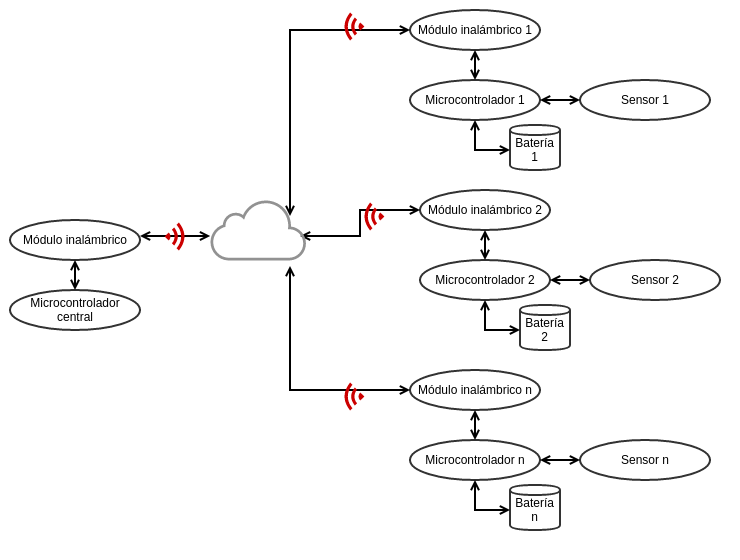
\includegraphics[width=.9\textwidth]{./Figuras/Figura1.png}
\caption{Diagrama en bloques del sistema}
\label{fig:diagBloques}
\end{figure}

\vspace{25px}

\end{consigna}




\section{Identificación y análisis de los interesados}
\label{sec:interesados}

\begin{consigna}{black} 

\begin{table}[ht]
%\caption{Identificación de los interesados}
%\label{tab:interesados}
\begin{tabularx}{\linewidth}{@{}|l|X|X|l|@{}}
\hline
\rowcolor[HTML]{C0C0C0} 
Rol           & Nombre y Apellido & Organización 	& Puesto 	\\ \hline
Cliente       & \clientename      &\empclientename	& CEO       \\ \hline
Responsable   & \authorname       & FIUBA        	& Alumno 	\\ \hline
Colaboradores & Raúl Palavecino   & -             	& Estudiante ingeniería electrónica       	\\ \hline
Orientador    & \supname	      & \pertesupname 	& Director	Trabajo final \\ \hline
Usuario final & Productores e \newline independientes \newline pequeña/mediana \newline escala. \newline Agricultura, \newline frutihortícola, plantas \newline ornamentales. Profesionales \newline dedicados a \newline climatizar \newline recintos para \newline diversos usos.                 & -             	& -       	\\ \hline
\end{tabularx}
\end{table}


\begin{itemize}
\item Cliente Pablo Lodeti: CEO de Wentux. Desarrolló el actual producto que tiene la empresa .
\item Colaborador Raúl Palavecino: Estudiante de la carrera ingeniería en electrónica y persona con experiencia en embebidos. 
\item Orientador Gonzalo Sanchez: Magister en sistema embebidos con experiencia en el microcontrolador a utilizar.
\end{itemize}

\end{consigna}



\section{1. Propósito del proyecto}
\label{sec:proposito}

\begin{consigna}{black}

El propósito del proyecto es desarrollar una red de sensores inalámbrica para eliminar las incomodidades y restricciones que genera el cableado actual que tienen los equipos. De esta forma, la nueva red de sensores inalámbrica beneficiará la instalación y la comodidad en el uso diario de los equipos.
\end{consigna}

\section{2. Alcance del proyecto}
\label{sec:alcance}

\begin{consigna}{black}
El proyecto incluye el desarrollo del firmware para la comunicación de los nodos con la central, prueba de prototipo  funcional y su puesta en funcionamiento en una pequeña  planta  dentro de las instalaciones del  taller o en  planta modelo  montada por colaborador  para pruebas, que simule el  invernadero a controlar. También se incluye el desarrollo del hardware del conjunto microcontrolador, sensor, batería y módulo inalámbrico (nodos). 

El proyecto no incluye la puesta en funcionamiento en campo y posterior mantenimiento .

\end{consigna}


\section{3. Supuestos del proyecto}
\label{sec:supuestos}

\begin{consigna}{black}

\begin{itemize}
\item El cliente proveerá los fondos para la compra de sensores,  actuadores y materiales varios para desarrollar la red de sensores.
\item El cliente deberá proveer un equipo funcionando con el cual la red de sensores deberá comunicarse.
\item El cliente proveerá un entorno o invernadero/indoor piloto de prueba.
\end{itemize}

\end{consigna}

\section{4. Requerimientos}
\label{sec:requerimientos}

\begin{consigna}{black}
Los requerimientos surgen del análisis realizado a la propuesta y relevamiento de proyecto que envía el cliente. Se detallan a continuación, agrupados por afinidad y se indica en cada uno su prioridad, siendo [0] la más alta y [3] la más baja.

\begin{enumerate}
\item Grupo de requerimientos asociados con comunicación
	\begin{enumerate}
	\item Cada nodo deberá enviar la información tomada del sensor a la central. El período de muestreo deberá ser configurable desde la central. Cada mensaje hacia la central tendrá un máximo de 10 bytes [0].
	\item Se deberá desarrollar un protocolo de comunicación entre la central y los nodos [0].
	\item Los nodos tendrán un sistema de reintento de envío de información a la central en caso de falla en la misma [2].
	\item Los nodos almacenarán en memoria interna información no enviada hasta que la misma se envíe en un reintento[3].
	\item La comunicación deberá estar protegida mediante un algoritmo de encriptación para que no sea alterada externamente [3].
	\end{enumerate}
\item Grupo de requerimientos asociados con alimentación
	\begin{enumerate}
	\item Los nodos estarán alimentados por batería como fuente eléctrica, el rango de tensión admisible será de 1.9v a 3.3v. La tensión nominal será de 3.3v. La batería deberá durar 30 días como mínimo [0].
	\item Se deberá desarrollar una función de ahorro de batería en los nodos [1].
	\end{enumerate}
\item Grupo de requerimientos asociados con generalidades del proyecto
	\begin{enumerate}
	\item Cada nodo estará compuesto por un conjunto de microcontrolador, módulo inalámbrico, sensor y batería. El sistema tendrá un máximo de 4 sensores y la distancia máxima a la central será de 15 metros [0].
	\item El sistema debe permitir instalarse en cualquier invernadero o indoor [2].
	\end{enumerate}
\item Grupo de requerimientos asociados con documentación y codificación
	\begin{enumerate}
	\item Se deberá entregar un manual de instalación y manual de uso [3].
	\item Se deberá usar Git como software de control de versiones [2].
	\item Se deberá documentar el código con doxygen [3].
	\end{enumerate}


\end{enumerate}

\end{consigna}

\section{Historias de usuarios (\textit{Product backlog})}
\label{sec:backlog}

\begin{consigna}{black}

Se enumeran las historias de usuario y su ponderación calculada en story points (del [1] al [5]).

\begin{enumerate}
\item Como usuario final del proyecto quiero poder visualizar la información obtenida de los sensores en tiempo real [2].

\item Como usuario final del producto quiero instalarlo de manera práctica, flexible y sin conocimiento técnico [1].

\item Como cliente del proyecto quiero eliminar el cableado del producto final [5].

\item Como cliente del proyecto quiero despreocuparme de la duración de las baterías [4].

\end{enumerate}


\end{consigna}

\section{5. Entregables principales del proyecto}
\label{sec:entregables}

\begin{consigna}{black}
Los entregables del proyecto son:

\begin{itemize}
\item Informe de avance
\item Manual de uso
\item Código fuente
\item Prototipo funcional
\item Manual de instalación
\item Memoria técnica

\end{itemize}

\end{consigna}

\section{6. Desglose del trabajo en tareas}
\label{sec:wbs}

\begin{consigna}{black}
El proyecto se divide en las siguientes tareas:

\begin{enumerate}
\item \textbf{Gestión del proyecto: 68 hs}
	\begin{enumerate}
	\item Planificación del proyecto (20 hs)
	\item Confección informe de avance (8 hs)
	\item Análisis y relevamiento inicial (15 hs)
	\item Confección manual de instalación (10 hs)
	\item Confección manual de uso (15 hs)
	\end{enumerate}
\item \textbf{Hardware: 42 hs}
	\begin{enumerate}
	\item Definición de componentes (7 hs)
	\item Compra de componentes (5 hs)
	\item Diseño de prototipos de los nodos (10 hs)
	\item Elaboración/construcción de los nodos (20 hs)
	\end{enumerate}
\item \textbf{Firmware: 238 hs}
	\begin{enumerate}
	\item Diseño de la solución (28 hs)
	\item Configuración de herramientas y plataforma de desarrollo (21 hs)
	\item Estudio y aprendizaje para el desarrollo de los componentes (20 hs)
	\item Desarrollo del protocolo de comunicación y su encriptación (40 hs)
	\item Desarrollo de la función ahorro de batería (33 hs)
	\item Desarrollo de configuración inicial de nuevo nodo en la red (35 hs)
	\item Desarrollo de los componentes de medición y almacenamiento (32 hs)
	\item Desarrollo del módulo de reenvío (29 hs)
	\end{enumerate}
\item \textbf{Testing y verificación: 115 hs}
	\begin{enumerate}
	\item Testing unitario del protocolo de comunicación (20 hs)
	\item Testing unitario de la función de ahorro de batería (15 hs)
	\item Testing unitario de nuevo nodo en red (18 hs)
	\item Testing unitario de la medición, almacenamiento y reenvío (25 hs)
	\item Testing de integración (37 hs)
	\end{enumerate}
\item \textbf{Implementación e integración: 50 hs}
	\begin{enumerate}
	\item Integración de los componentes con un producto final (20 hs)
	\item Implementación del prototipo en una planta real (indoor o invernadero) (30 hs)
	\end{enumerate}
\item \textbf{Presentación del trabajo: 90 hs}
	\begin{enumerate}
	\item Confección de la memoria (70 hs)
	\item Preparación de la presentación final (20 hs)
	\end{enumerate}
\end{enumerate}

\textbf{Cantidad total de horas: (603 hs)}


\end{consigna}

\section{7. Diagrama de Activity On Node}
\label{sec:AoN}

\begin{consigna}{black}

En la Figura \ref{fig:aon} se detalla el diagrama de Activity On Node asociado a las tareas del proyecto. Los colores representan las agrupaciones que se realizaron en el desglose del trabajo en tareas, estas son:

\begin{enumerate}
	\item Gestión del proyecto (celeste)
	\item Hardware (lila)
	\item Firmware (colorado)
	\item Testing y verificación (amarillo)
	\item Implementación e integración (verde)
	\item Presentación del trabajo (gris)
\end{enumerate}

%La figura \ref{fig:AoN} fue elaborada con el paquete latex tikz y pueden consultar la siguiente referencia \textit{online}:

%\url{https://www.overleaf.com/learn/latex/LaTeX_Graphics_using_TikZ:_A_Tutorial_for_Beginners_(Part_3)\%E2\%80\%94Creating_Flowcharts}

\end{consigna}

\begin{figure}[htpb]
\centering 
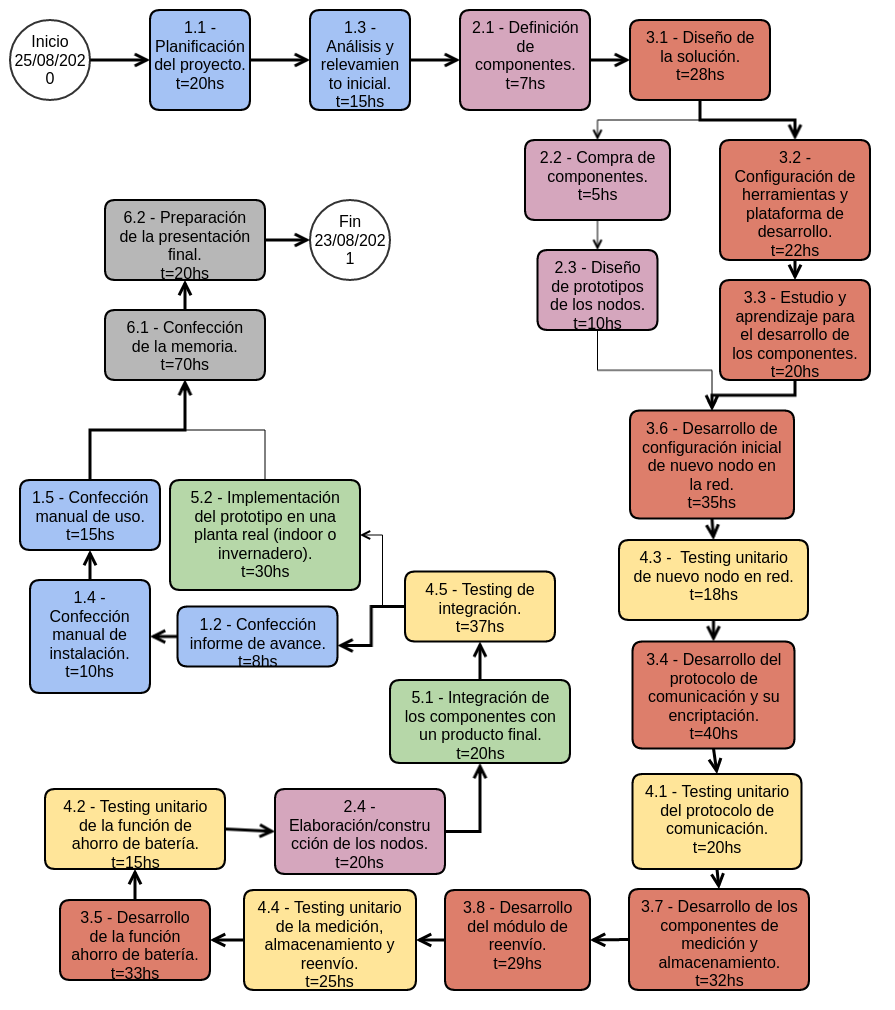
\includegraphics[width=.9\textwidth]{./Figuras/aon.png}
\caption{Diagrama en \textit{Activity on Node}}
\label{fig:aon}
\end{figure}



\section{8. Diagrama de Gantt}
\label{sec:gantt}

\begin{consigna}{red}
Utilizar el software Gantter for Google Drive o alguno similar para dibujar el diagrama de Gantt.

Existen muchos programas y recursos \textit{online} para hacer diagramas de gantt, entre las cuales destacamos:

\begin{itemize}
\item Planner
\item GanttProject
\item Trello + \textit{plugins}. En el siguiente link hay un tutorial oficial: \\ \url{https://blog.trello.com/es/diagrama-de-gantt-de-un-proyecto}
\item Creately, herramienta online colaborativa. \\\url{https://creately.com/diagram/example/ieb3p3ml/LaTeX}
\item Se puede hacer en latex con el paquete \textit{pgfgantt}\\ \url{http://ctan.dcc.uchile.cl/graphics/pgf/contrib/pgfgantt/pgfgantt.pdf}
\end{itemize}

Pegar acá una captura de pantalla del diagrama de Gantt, cuidando que la letra sea suficientemente grande como para ser legible. 
Si el diagrama queda demasiado ancho, se puede pegar primero la ``tabla'' del Gantt y luego pegar la parte del diagrama de barras del diagrama de Gantt.

Configurar el software para que en la parte de la tabla muestre los códigos del EDT (WBS).\\
Configurar el software para que al lado de cada barra muestre el nombre de cada tarea.\\
Revisar que la fecha de finalización coincida con lo indicado en el Acta Constitutiva.

En la figura \ref{fig:gantt}, se muestra un ejemplo de diagrama de gantt realizado con el paquete de \textit{pgfgantt}. En la plantilla pueden ver el código que lo genera y usarlo de base para construir el propio.

\begin{figure}[htbp]
\begin{center}
\begin{ganttchart}{1}{12}
  \gantttitle{2020}{12} \\
  \gantttitlelist{1,...,12}{1} \\
  \ganttgroup{Group 1}{1}{7} \\
  \ganttbar{Task 1}{1}{2} \\
  \ganttlinkedbar{Task 2}{3}{7} \ganttnewline
  \ganttmilestone{Milestone o hito}{7} \ganttnewline
  \ganttbar{Final Task}{8}{12}
  \ganttlink{elem2}{elem3}
  \ganttlink{elem3}{elem4}
\end{ganttchart}
\end{center}
\caption{Diagrama de gantt de ejemplo}
\label{fig:gantt}
\end{figure}

\end{consigna}

\section{9. Matriz de uso de recursos de materiales}
\label{sec:recursos}


\begin{table}
\label{tab:recursos}
\centering
\begin{tabularx}{\linewidth}{@{}|c|X|X|X|X|c|@{}}
\hline
\cellcolor[HTML]{C0C0C0} & \cellcolor[HTML]{C0C0C0} & \multicolumn{4}{c|}{\cellcolor[HTML]{C0C0C0}Recursos requeridos (horas)} \\ \cline{3-6} 
\multirow{-2}{*}{\cellcolor[HTML]{C0C0C0}\begin{tabular}[c]{@{}c@{}}Código\\ WBS\end{tabular}} & \multirow{-2}{*}{\cellcolor[HTML]{C0C0C0}\begin{tabular}[c]{@{}c@{}}Nombre \\ tarea\end{tabular}} & Material 1 & Material 2 & Material 3 & Material 4 \\ \hline
 &  &  &  &  &  \\ \hline
 &  &  &  &  &  \\ \hline
 &  &  &  &  &  \\ \hline
 &  &  &  &  &  \\ \hline
 &  &  &  &  &  \\ \hline
 &  &  &  &  &  \\ \hline
 &  &  &  &  &  \\ \hline
 &  &  &  &  &  \\ \hline 
 &  &  &  &  &  \\ \hline
 &  &  &  &  &  \\ \hline
 &  &  &  &  &  \\ \hline
 &  &  &  &  &  \\ \hline
 &  &  &  &  &  \\ \hline
 &  &  &  &  &  \\ \hline
 &  &  &  &  &  \\ \hline
 &  &  &  &  &  \\ \hline
 &  &  &  &  &  \\ \hline
 &  &  &  &  &  \\ \hline
 &  &  &  &  &  \\ \hline
 &  &  &  &  &  \\ \hline
 &  &  &  &  &  \\ \hline
 &  &  &  &  &  \\ \hline
 &  &  &  &  &  \\ \hline
 &  &  &  &  &  \\ \hline 
 &  &  &  &  &  \\ \hline
 &  &  &  &  &  \\ \hline
 &  &  &  &  &  \\ \hline
 &  &  &  &  &  \\ \hline

\end{tabularx}%
\end{table}


\section{10. Presupuesto detallado del proyecto}
\label{sec:presupuesto}

\begin{consigna}{red}
Si el proyecto es complejo entonces separarlo en partes:
\begin{itemize}
\item Un total global, indicando el subtotal acumulado por cada una de las áreas.
\item El desglose detallado del subtotal de cada una de las áreas.
\end{itemize}

IMPORTANTE: No olvidarse de considerar los COSTOS INDIRECTOS.

\end{consigna}

\begin{table}[htpb]
\centering
\begin{tabularx}{\linewidth}{@{}|X|c|r|r|@{}}
\hline
\rowcolor[HTML]{C0C0C0} 
\multicolumn{4}{|c|}{\cellcolor[HTML]{C0C0C0}COSTOS DIRECTOS} \\ \hline
\rowcolor[HTML]{C0C0C0} 
Descripción &
  \multicolumn{1}{c|}{\cellcolor[HTML]{C0C0C0}Cantidad} &
  \multicolumn{1}{c|}{\cellcolor[HTML]{C0C0C0}Valor unitario} &
  \multicolumn{1}{c|}{\cellcolor[HTML]{C0C0C0}Valor total} \\ \hline
 &
  \multicolumn{1}{c|}{} &
  \multicolumn{1}{c|}{} &
  \multicolumn{1}{c|}{} \\ \hline
 &
  \multicolumn{1}{c|}{} &
  \multicolumn{1}{c|}{} &
  \multicolumn{1}{c|}{} \\ \hline
\multicolumn{1}{|l|}{} &
   &
   &
   \\ \hline
\multicolumn{1}{|l|}{} &
   &
   &
   \\ \hline
\multicolumn{3}{|c|}{SUBTOTAL} &
  \multicolumn{1}{c|}{} \\ \hline
\rowcolor[HTML]{C0C0C0} 
\multicolumn{4}{|c|}{\cellcolor[HTML]{C0C0C0}COSTOS INDIRECTOS} \\ \hline
\rowcolor[HTML]{C0C0C0} 
Descripción &
  \multicolumn{1}{c|}{\cellcolor[HTML]{C0C0C0}Cantidad} &
  \multicolumn{1}{c|}{\cellcolor[HTML]{C0C0C0}Valor unitario} &
  \multicolumn{1}{c|}{\cellcolor[HTML]{C0C0C0}Valor total} \\ \hline
\multicolumn{1}{|l|}{} &
   &
   &
   \\ \hline
\multicolumn{1}{|l|}{} &
   &
   &
   \\ \hline
\multicolumn{1}{|l|}{} &
   &
   &
   \\ \hline
\multicolumn{3}{|c|}{SUBTOTAL} &
  \multicolumn{1}{c|}{} \\ \hline
\rowcolor[HTML]{C0C0C0}
\multicolumn{3}{|c|}{TOTAL} &
   \\ \hline
\end{tabularx}%
\end{table}


\section{11. Matriz de asignación de responsabilidades}
\label{sec:responsabilidades}
\begin{consigna}{red}
Establecer la matriz de asignación de responsabilidades y el manejo de la autoridad completando la siguiente tabla:

\begin{table}[htpb]
\centering
\resizebox{\textwidth}{!}{%
\begin{tabular}{|c|c|c|c|c|c|}
\hline
\rowcolor[HTML]{C0C0C0} 
\cellcolor[HTML]{C0C0C0} &
  \cellcolor[HTML]{C0C0C0} &
  \multicolumn{4}{c|}{\cellcolor[HTML]{C0C0C0}Listar todos los nombres y roles del proyecto} \\ \cline{3-6} 
\rowcolor[HTML]{C0C0C0} 
\cellcolor[HTML]{C0C0C0} &
  \cellcolor[HTML]{C0C0C0} &
  Responsable &
  Orientador &
  Equipo &
  Cliente \\ \cline{3-6} 
\rowcolor[HTML]{C0C0C0} 
\multirow{-3}{*}{\cellcolor[HTML]{C0C0C0}\begin{tabular}[c]{@{}c@{}}Código\\ WBS\end{tabular}} &
  \multirow{-3}{*}{\cellcolor[HTML]{C0C0C0}Nombre de la tarea} &
  \authorname &
  \supname &
  Nombre de alguien &
  \clientename \\ \hline
 &  &  &  &  &  \\ \hline
 &  &  &  &  &  \\ \hline
 &  &  &  &  &  \\ \hline
\end{tabular}%
}
\end{table}

{\footnotesize
Referencias:
\begin{itemize}
	\item P = Responsabilidad Primaria
	\item S = Responsabilidad Secundaria
	\item A = Aprobación
	\item I = Informado
	\item C = Consultado
\end{itemize}
} %footnotesize

Una de las columnas debe ser para el Director, ya que se supone que participará en el proyecto.
A su vez se debe cuidar que no queden muchas tareas seguidas sin ``A'' o ``I''.

Importante: es redundante poner ``I/A'' o ``I/C'', porque para aprobarlo o responder consultas primero la persona debe ser informada.

\end{consigna}

\section{12. Gestión de riesgos}
\label{sec:riesgos}

\begin{consigna}{red}
a) Identificación de los riesgos (al menos cinco) y estimación de sus consecuencias:
 
Riesgo 1: detallar el riesgo (riesgo es algo que si ocurre altera los planes previstos)
\begin{itemize}
\item Severidad (S): mientras más severo, más alto es el número (usar números del 1 al 10).\\
Justificar el motivo por el cual se asigna determinado número de severidad (S).
\item Probabilidad de ocurrencia (O): mientras más probable, más alto es el número (usar del 1 al 10).\\
Justificar el motivo por el cual se asigna determinado número de (O). 
\end{itemize}   

Riesgo 2:
\begin{itemize}
\item Severidad (S): 
\item Ocurrencia (O):
\end{itemize}

Riesgo 3:
\begin{itemize}
\item Severidad (S): 
\item Ocurrencia (O):
\end{itemize}


b) Tabla de gestión de riesgos:      (El RPN se calcula como RPN=SxO)

\begin{table}[htpb]
\centering
\begin{tabularx}{\linewidth}{@{}|X|c|c|c|c|c|c|@{}}
\hline
\rowcolor[HTML]{C0C0C0} 
Riesgo & S & O & RPN & S* & O* & RPN* \\ \hline
       &   &   &     &    &    &      \\ \hline
       &   &   &     &    &    &      \\ \hline
       &   &   &     &    &    &      \\ \hline
       &   &   &     &    &    &      \\ \hline
       &   &   &     &    &    &      \\ \hline
\end{tabularx}%
\end{table}

Criterio adoptado: 
Se tomarán medidas de mitigación en los riesgos cuyos números de RPN sean mayores a...

Nota: los valores marcados con (*) en la tabla corresponden luego de haber aplicado la mitigación.

c) Plan de mitigación de los riesgos que originalmente excedían el RPN máximo establecido:
 
Riesgo 1: plan de mitigación (si por el RPN fuera necesario elaborar un plan de mitigación).
  Nueva asignación de S y O, con su respectiva justificación:
  - Severidad (S): mientras más severo, más alto es el número (usar números del 1 al 10).
          Justificar el motivo por el cual se asigna determinado número de severidad (S).
  - Probabilidad de ocurrencia (O): mientras más probable, más alto es el número (usar del 1 al 10).
          Justificar el motivo por el cual se asigna determinado número de (O).

Riesgo 2: plan de mitigación (si por el RPN fuera necesario elaborar un plan de mitigación).
 
Riesgo 3: plan de mitigación (si por el RPN fuera necesario elaborar un plan de mitigación).

\end{consigna}


\section{13. Gestión de la calidad}
\label{sec:calidad}

\begin{consigna}{red}
Para cada uno de los requerimientos del proyecto indique:
\begin{itemize} 
\item Req \#1: copiar acá el requerimiento.

Verificación y validación:

\begin{itemize}
\item Verificación para confirmar si se cumplió con lo requerido antes de mostrar el sistema al cliente. Detallar 
\item Validación con el cliente para confirmar que está de acuerdo en que se cumplió con lo requerido. Detallar  
\end{itemize}

\end{itemize}

Tener en cuenta que en este contexto se pueden mencionar simulaciones, cálculos, revisión de hojas de datos, consulta con expertos, mediciones, etc.

\end{consigna}

\section{14. Comunicación del proyecto}
\label{sec:comunicaciones}

El plan de comunicación del proyecto es el siguiente:

\begin{table}[htpb]
\centering
\begin{tabularx}{\linewidth}{@{}|X|C{2.4cm}|C{3cm}|C{1.8cm}|C{2cm}|C{2.1cm}|@{}}
\hline
\rowcolor[HTML]{C0C0C0} 
\multicolumn{6}{|c|}{\cellcolor[HTML]{C0C0C0}PLAN DE COMUNICACIÓN DEL PROYECTO}           \\ \hline
\rowcolor[HTML]{C0C0C0} 
¿Qué comunicar? & Audiencia & Propósito & Frecuencia & Método de comunicac. & Responsable \\ \hline
                &           &           &            &                      &             \\ \hline
                &           &           &            &                      &             \\ \hline
                &           &           &            &                      &             \\ \hline
                &           &           &            &                      &             \\ \hline
                &           &           &            &                      &             \\ \hline
\end{tabularx}
\end{table}

\section{15. Gestión de compras}
\label{sec:compras}

\begin{consigna}{red}
En caso de tener que comprar elementos o contratar servicios:
a) Explique con qué criterios elegiría a un proveedor.
b) Redacte el Statement of Work correspondiente.
\end{consigna}

\section{16. Seguimiento y control}
\label{sec:seguimiento}

\begin{consigna}{red}
Para cada tarea del proyecto establecer la frecuencia y los indicadores con los se seguirá su avance y quién será el responsable de hacer dicho seguimiento y a quién debe comunicarse la situación (en concordancia con el Plan de Comunicación del proyecto).

El indicador de avance tiene que ser algo medible, mejor incluso si se puede medir en \% de avance. Por ejemplo,se pueden indicar en esta columna cosas como ``cantidad de conexiones ruteadeas'' o ``cantidad de funciones implementadas'', pero no algo genérico y ambiguo como ``\%'', porque el lector no sabe porcentaje de qué cosa.

\end{consigna}

\begin{longtable}{|m{1cm}|m{3.5cm}|m{2.2cm}|m{2cm}|m{3cm}|m{1.5cm}|}
\hline
\rowcolor[HTML]{C0C0C0} 
\multicolumn{6}{|c|}{\cellcolor[HTML]{C0C0C0}SEGUIMIENTO DE AVANCE}                                                                       \\ \hline
\rowcolor[HTML]{C0C0C0} 
Tarea del WBS 			& Indicador de avance & Frecuencia de reporte & Resp. de seguimiento & Persona a ser informada & Método de comunic. \\ \hline
\endfirsthead

\hline
\rowcolor[HTML]{C0C0C0} 
\multicolumn{6}{c}{\cellcolor[HTML]{C0C0C0}SEGUIMIENTO DE AVANCE}                                                                       \\ \hline
\rowcolor[HTML]{C0C0C0} 
Tarea del WBS 			& Indicador de avance & Frecuencia de reporte & Resp. de seguimiento & Persona a ser informada & Método de comunic. \\ \hline
\endhead

\multicolumn{6}{c}{Continúa}
\endfoot

\endlastfoot

1.1	& Fecha de inicio  & Única vez al comienzo & \authorname & \clientename, \supname & email \\ \hline
2.1	& Avance de las subtareas  & Mensual mientras dure la tarea & \authorname & \clientename, \supname & email \\ \hline

\end{longtable}

\begin{table}[!htpb]
\centering
%\begin{tabularx}{\linewidth}{@{}|X|X|X|X|X|X|@{}}
\begin{tabularx}{\linewidth}{@{}|X|C{2.5cm}|C{3cm}|C{2cm}|C{2cm}|C{2.5cm}|@{}}
\hline
\rowcolor[HTML]{C0C0C0} 
\multicolumn{6}{|c|}{\cellcolor[HTML]{C0C0C0}SEGUIMIENTO DE AVANCE}                                                                       \\ \hline
\rowcolor[HTML]{C0C0C0} 
Tarea del WBS & Indicador de avance & Frecuencia de reporte & Resp. de seguimiento & Persona a ser informada & Método de comunic. \\ \hline
 &  &  &  &  &  \\ \hline
 &  &  &  &  &  \\ \hline
 &  &  &  &  &  \\ \hline
 &  &  &  &  &  \\ \hline
 &  &  &  &  &  \\ \hline
\end{tabularx}%
%}
\end{table}

\section{17. Procesos de cierre}    
\label{sec:cierre}

\begin{consigna}{red}
Establecer las pautas de trabajo para realizar una reunión final de evaluación del proyecto, tal que contemple las siguientes actividades:

\begin{itemize}
\item Pautas de trabajo que se seguirán para analizar si se respetó el Plan de Proyecto original:
 - Indicar quién se ocupará de hacer esto y cuál será el procedimiento a aplicar. 
\item Identificación de las técnicas y procedimientos útiles e inútiles que se utilizaron, y los problemas que surgieron y cómo se solucionaron:
 - Indicar quién se ocupará de hacer esto y cuál será el procedimiento para dejar registro.
\item Indicar quién organizará el acto de agradecimiento a todos los interesados, y en especial al equipo de trabajo y colaboradores:
  - Indicar esto y quién financiará los gastos correspondientes.
\end{itemize}

\end{consigna}


\end{document}
